\section{Businesses}
	\subsection{Registration}
	If you want to create a business account for \textit{Soldino}, visit the 
	homepage, make sure you are logged in your MetaMask\glosp account and
	then make sure that the switch button is set on \texttt{Business}.\\
	\begin{figure}[H]
		
\includegraphics[width=5cm]{res/images/user_business.png}
		\centering
		\caption{Select \texttt{Business} from the switch button}
	\end{figure}	
	\noindent Then, insert your business' data in the form.
	\begin{figure}[H]
		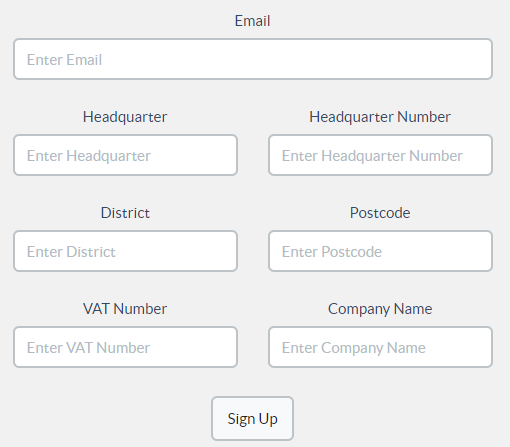
\includegraphics[width=10cm]{res/images/business_signup.png}
		\centering
		\caption{Business sign up form}
	\end{figure}
	\noindent After you have completed 
	all the	fields with your informations, press the \texttt{Sign up} button. If an 
	entry is not valid (e.g. the email address does not contain a valid 
	domain), the system will let you know and you have to correct that field 
	to continue. If all informations are correct, a pop-up window will open 
	asking you to allow \textit{Soldino} to access your information.\\
	\begin{figure}[H]
		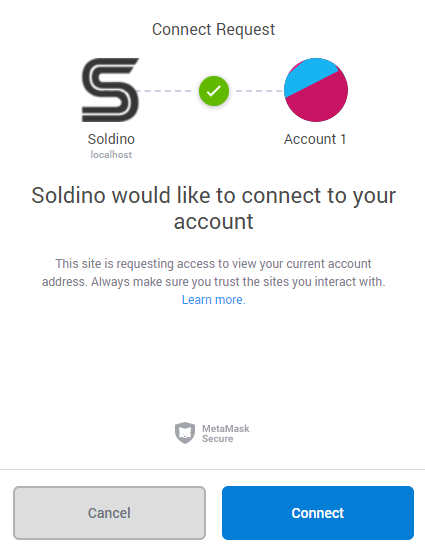
\includegraphics[width=10cm]{res/images/metamask_connect.png}
		\centering
		\caption{Connecting MetaMask to \textit{Soldino}}
	\end{figure}
	\noindent \noindent Press \texttt{Connect} and you will be redirected to a page 
	congratulating you for your registration on the platform.
	\begin{figure}[H]
		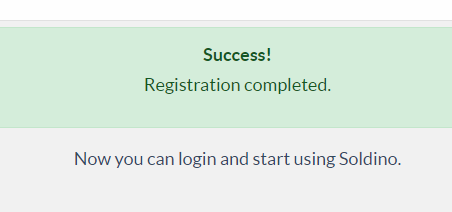
\includegraphics[width=10cm]{res/images/registration_complete.png}
		\centering
		\caption{Registration is completed message}
	\end{figure}
		\subsubsection{Business is already registered}
		If your Ethereum\glosp address is already registered in the platform, you will 
		see an error message.
		\begin{figure}[H]
			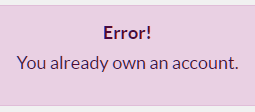
\includegraphics[width=10cm]{res/images/user_already_registered.png}
			\centering
			\caption{Error shown if you are already registered}
		\end{figure}
		\noindent Just press \texttt{Login} to log in your business account.
	\subsection{Login}
	If you already have a business account press the \texttt{Login} button on the 
	top right of the homepage, you will automatically log in your account 
	(there is no need for an username or password, all data are done via MetaMask). 
	\\To be able to log in you have to be logged in your MetaMask\glosp account.
		\subsubsection{Account is disabled}
		If your account was disabled by the Government, you will see an error 
		message.
		\begin{figure}[H]
			
\includegraphics[width=10cm]{res/images/user_disabled.png}
			\centering
			\caption{Error shown if your account has been disabled by the Government}
		\end{figure}
	\noindent If your account is disabled, you cannot access it any more until it 
	is enabled again by the Government.
	\subsection{Logout}
	To log out of \textit{Soldino} you just have to log out of 
	MetaMask\glo{}. To do this, you have to press MetaMask's icon on the top 
	right of the browser, press your account's icon and then press \texttt{Log out}
	on the top right.
	\begin{figure}[H]
		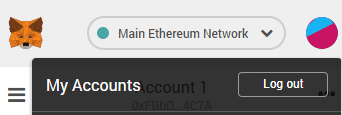
\includegraphics[width=10cm]{res/images/logout_metamask.png}
		\centering
		\caption{Logging out}
	\end{figure}
	\subsection{Buying}
	After completing the login, you will be redirected in the store main page. 
	Here you will find some of the products and the search bar.
	\begin{figure}[H]
		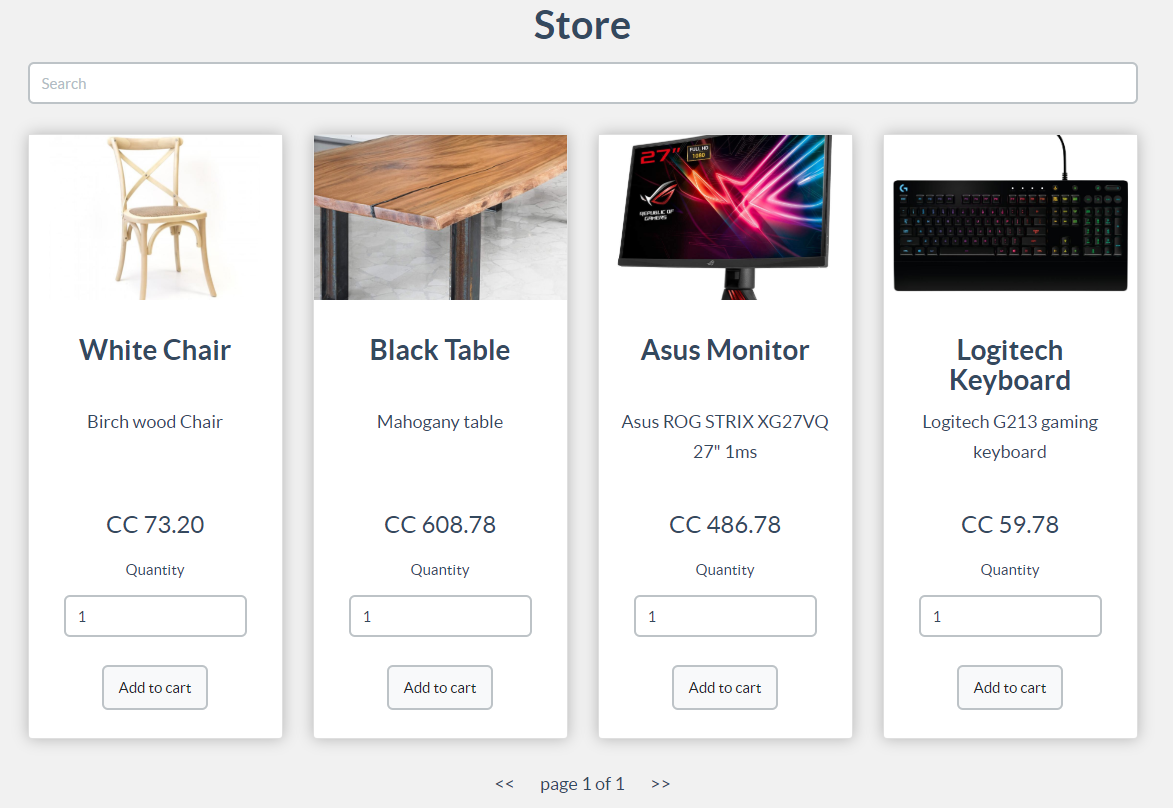
\includegraphics[width=15cm]{res/images/store_main_page.png}
		\centering
		\caption{Store front page}
	\end{figure}
	\noindent Note that all prices shown in the platform are in Cubits\glosp (CC\glo), 
	\textit{Soldino}'s own special token. Also, note that 1 Cubit equals 1 Euro.
		\subsubsection{Searching}
		You can search for products by name using the search bar that can be 
		found on the top of the page. Pay attention you can use the search bar 
		to find products by words that are in their titles only. \\
		After you start typing you will see 
		all results that match your search. If no matching products are 
		found, a message will be shown.
%		
		\subsubsection{Cart}
		You can add products in your cart, after selecting the quantity you need, 
		by pressing the \texttt{Add to cart} button under it.
	\begin{figure}[H]
		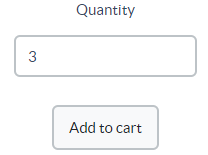
\includegraphics[width=7cm]{res/images/add_to_cart.png}
		\centering
		\caption{Adding a product to the cart}
	\end{figure}
	\noindent The number on the cart shows you how many unique products are 
	in it. You can access your cart by pressing the shopping cart icon in 
	the navigation bar at the top of the page.
	\begin{figure}[H]
		
\includegraphics[width=3cm]{res/images/cart_icon.png}
		\centering
		\caption{Shopping cart icon}
	\end{figure}
	\noindent Here you will see the total for your order and you will find 
	every item you have previously selected with their quantity. If you 
	need to modify the quantity press the \texttt{+} or \texttt{-} buttons.
	\begin{figure}[H]
		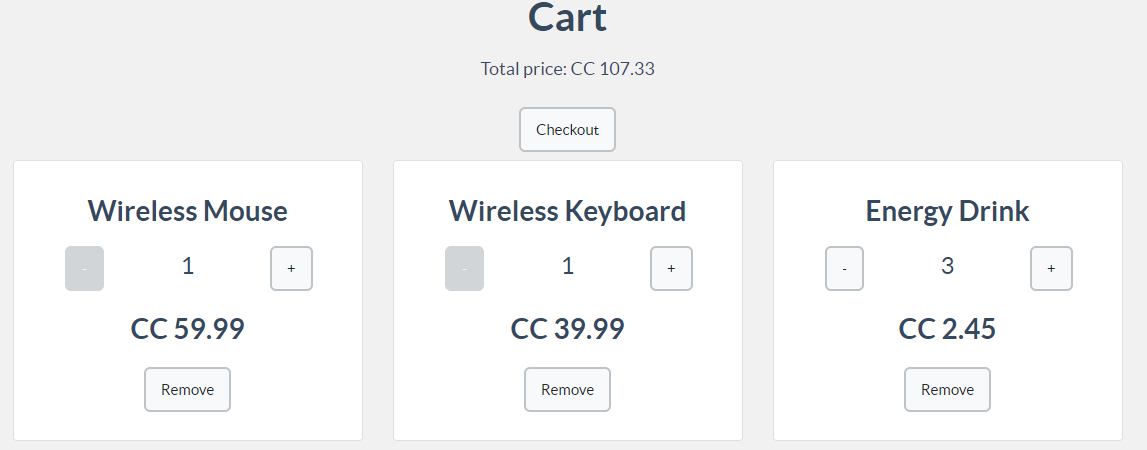
\includegraphics[width=15cm]{res/images/cart_example.png}
		\centering
		\caption{Example of a cart's content}
	\end{figure}
	\noindent When you want to proceed with the order, press the \texttt{Checkout} button. 
	You will be redirected to the checkout page.
		\subsubsection{Checkout}
		In the checkout page, you will be able to choose where your products 
		will be delivered to by using the radio buttons: you can either select 
		the address you gave during registration or enter a new one.
	\begin{figure}[H]
		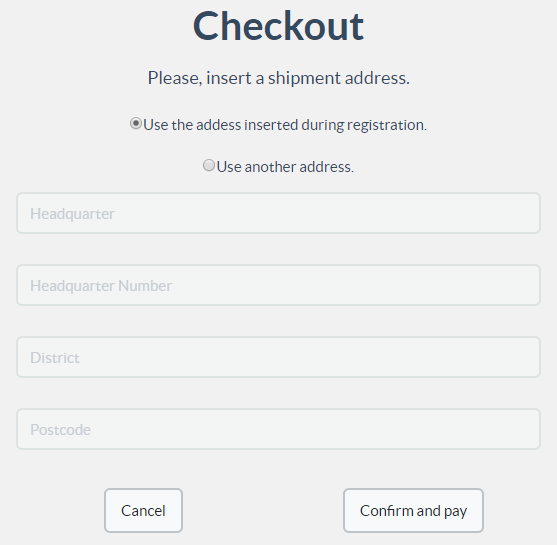
\includegraphics[width=10cm]{res/images/checkout.png}
		\centering
		\caption{Example of a checkout page}
	\end{figure}
	\noindent Press the \texttt{Confirm and pay} button to proceed. In a new 
	MetaMask\glo{} pop up window, press \texttt{Confirm} to be able to pay all the 
	vendors of the products that you are buying in just one transaction. After this 
	a new MetaMask\glo{} window will ask you to confirm the transaction showing you 
	the total cost of your order. Press \texttt{Confirm} to pay or press \texttt{Cancel}
	button if you do not want to continue.
		\subsubsection{Past orders}
		You can visit the page containing all past orders by pressing the 
		\texttt{Orders} button in the bar at the top of the page.
		Here you will find a order history where there is every purchase that you made 
		with \textit{Soldino}. Each order tells when it was made, who was the 
		seller, what were the items bought, where it was shipped to and how 
		much you paid for it.
		\begin{figure}[H]
			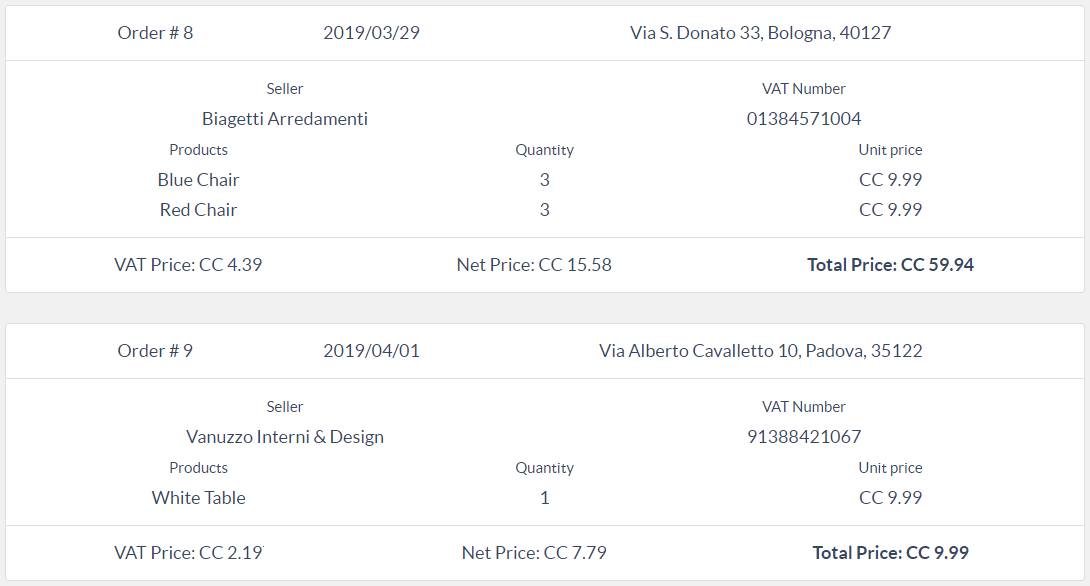
\includegraphics[width=15cm]{res/images/past_orders.png}
			\centering
			\caption{Example of past orders}
		\end{figure}
	\subsection{Selling}
	If you want to manage the products that you are selling on \textit{Soldino} 
	or add a new one, you have to press the \texttt{Products Manager} on the bar at the 
	top of the page. Here you will find every product that you are currently selling.
	\begin{figure}[H]
		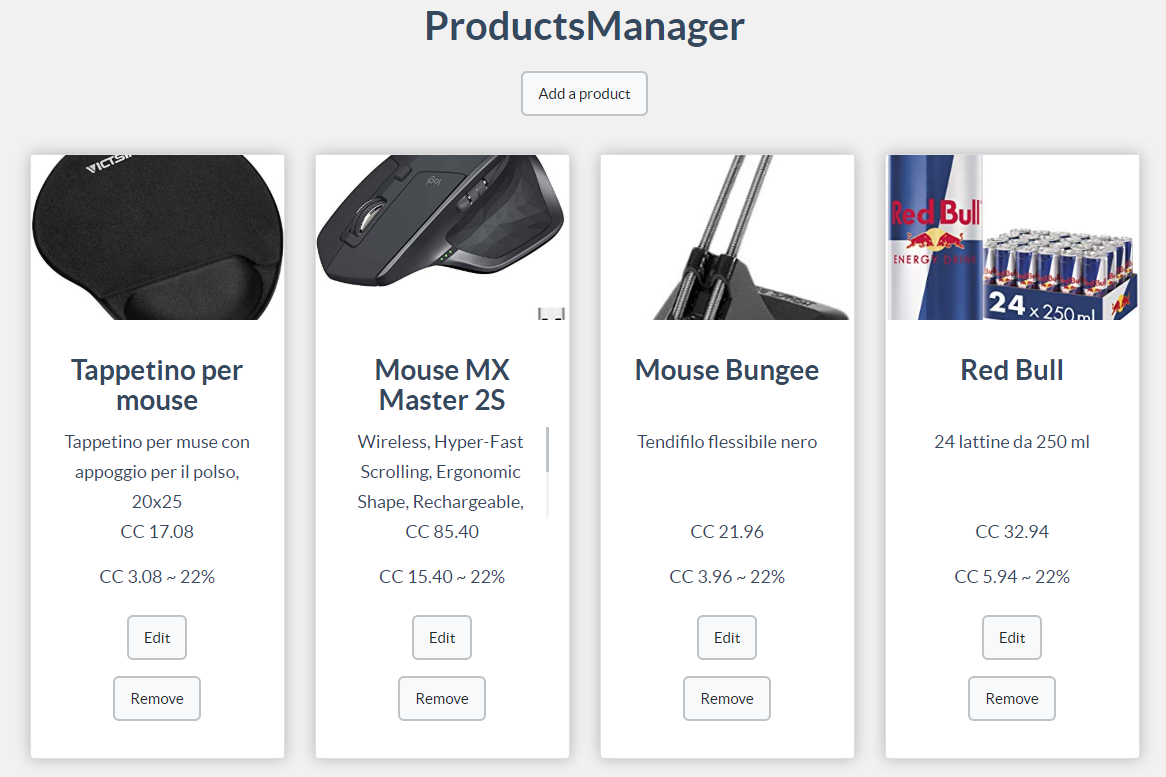
\includegraphics[width=15cm]{res/images/products_manager.png}
		\centering
		\caption{Products Manager page}
	\end{figure}
		\subsubsection{Selling a new product}
		If you want to sell a new product, you have to press \texttt{Add a product}, you 
		will be redirected to a page where you will have to insert all the 
		informations about your new product.
		\begin{figure}[H]
			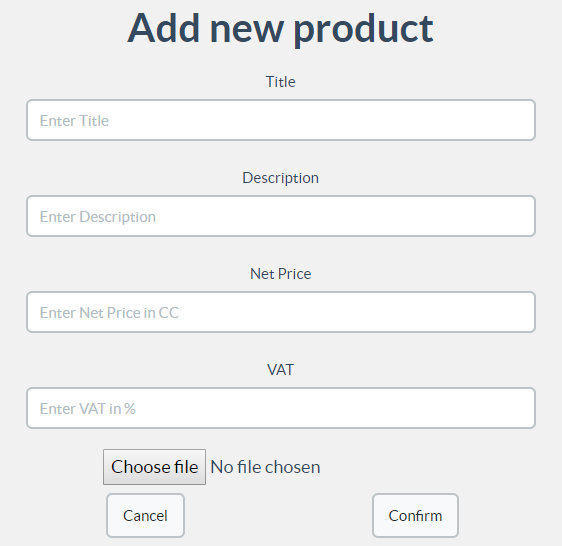
\includegraphics[width=10cm]{res/images/add_new_product.png}
			\centering
			\caption{Adding a new product}
		\end{figure}
		\noindent After you completed every field and you selected a photo 
		(adding a photo shall not be required, but it is recommended),
		press \texttt{Confirm} button and 
		it will be added to the products that users can buy.
		\\Press \texttt{Cancel} button if you do not wish to continue.
		\\Note that the photo must be a .png, .jpg or .gif file and the 
		 choosen picture could be for illustrative purposes only.
		 
		\subsubsection{Editing a product}
		If you want to change the information of a product, you have to press
		the \texttt{Edit} button and then you will be redirected to a 
		page where you will be able to change the product's information.
		\begin{figure}[H]
			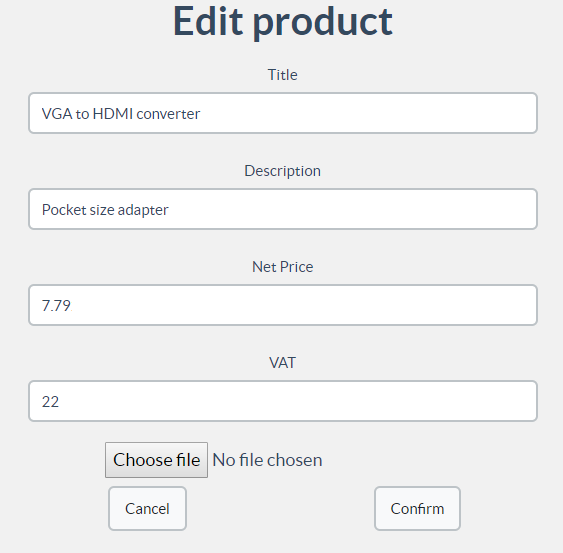
\includegraphics[width=10cm]{res/images/edit_product.png}
			\centering
			\caption{Editing the product's information}
		\end{figure}
		\noindent After you are done with the changes press the \texttt{Confirm} 
		button to apply them.\\
		Note that you have to insert only the fields you wish to change, leaving
		 the others blank.
		\\If you do not wish to apply the changes, press the \texttt{Cancel} button.
		\subsubsection{Removing a product}
		If you want to remove a product that you are selling on the platform, press 
		the	\texttt{Remove} button under it.
		\\Note that removing a product will not delete it from orders previously made. 
	\subsection{VAT management}
	If you are a business, \textit{Soldino} will manage VAT for the products 
	you buy and sell on the platform automatically. You can access the page 
	containing all invoices by pressing the \texttt{Transaction Manager} button 
	in the navigation bar at the top of the page.
	\begin{figure}[H]
		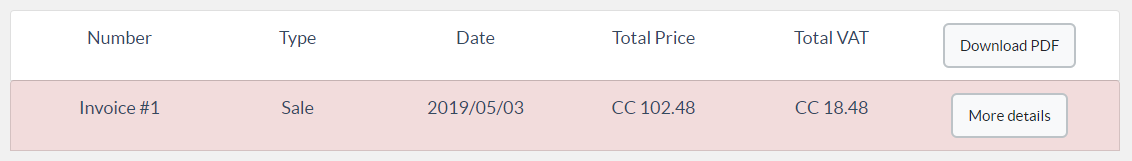
\includegraphics[width=15cm]{res/images/past_invoices.png}
		\centering
		\caption{Example of past invoices}
	\end{figure}
	\noindent Here you will also see the status of the quarter. 
	\\A red value at the end of a quarter means that you will have to pay 
	that amount to the Government.
	\begin{figure}[H]
		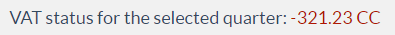
\includegraphics[width=10cm]{res/images/negative_vat_status.png}
		\centering
		\caption{Example of VAT input status}
	\end{figure}
	\noindent While a green one means that you will 
	soon be reimbursed for that amount.
	\begin{figure}[H]
		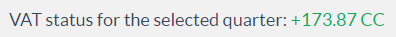
\includegraphics[width=10cm]{res/images/positive_vat_status.png}
		\centering
		\caption{Example of VAT output status}
	\end{figure}
		\subsubsection{Invoices}
		You can see more information about an invoice by pressing the 
		\texttt{More details} button. This will open a pop-up window containing all 
		the details.
		\begin{figure}[H]
			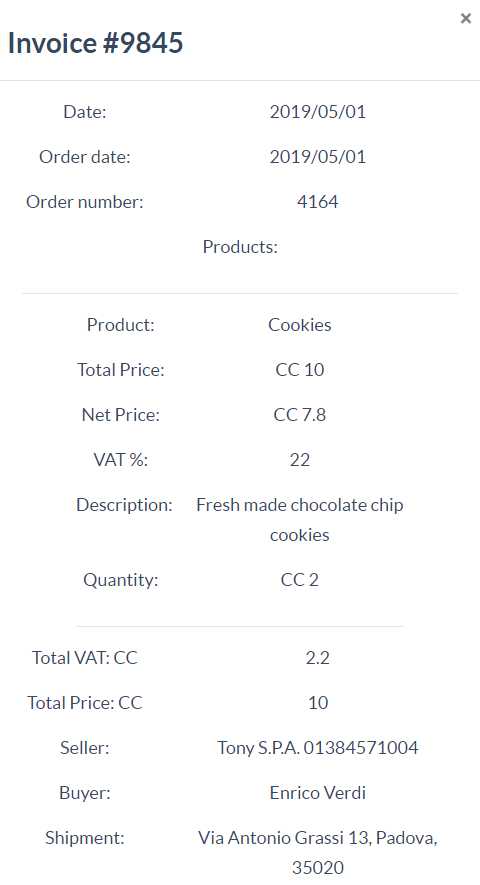
\includegraphics[width=10cm]{res/images/invoice_details.png}
			\centering
			\caption{Example of an invoice}
		\end{figure}
		\noindent You can also download a PDF file containing all the invoices 
		of this trimester by pressing \texttt{Download PDF}. 
		\subsubsection{Paying VAT}
		At the end of a quarter, if you are in debit with the government, next 
		to how much you have to pay you will see two buttons.
		\begin{figure}[H]
			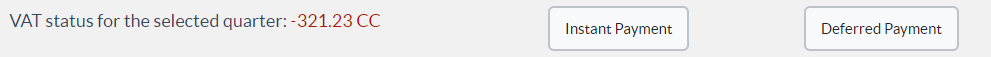
\includegraphics[width=15cm]{res/images/paying_vat.png}
			\centering
			\caption{Paying off Vat input status}
		\end{figure}
			\paragraph{Instant payment} \mbox{}\\
			If you choose to instantly pay off what you owe, press the \texttt{Instant 
			payment} button. MetaMask\glosp then will open a new window asking you to allow the 
			transaction and you have to accept to continue.
			\paragraph{Deferred payment} \mbox{}\\
			Otherwise, you can choose defererred payment\glosp by pressing the \texttt{Deferred payment} button.
%
		\subsubsection{Checking past quarters' VAT}
		You can see invoices of past quarters by using the drop-down 
		menu at the top of the page.
		\begin{figure}[H]
			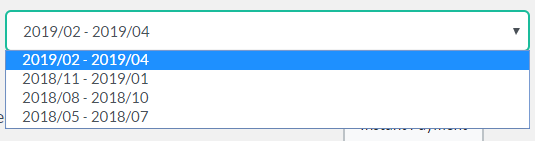
\includegraphics[width=10cm]{res/images/past_trimesters.png}
			\centering
			\caption{Past trimesters}
		\end{figure}
		\noindent From this page you will also be able to see specific details 
		of an invoice or download them all as PDF as explained before.